\clearpage
\section{Previous searches}
\label{sec:previous-searches}

Since Higgsinos provide solutions to puzzles and shortcomings in the SM, there have been numerous attempts to discover them at the LHC and previous colliders. These searches have led to exclusion limits on the available parameter space, as no supersymmetric particle has been found to date. Given the various possible final states or signatures associated with Higgsino production, the following summary focuses on searches that share similar phase space and final states with the present study. Specifically, searches of interest involve final states with leptons resulting from the prompt decay of electroweakinos.

Constraints on these compressed scenarios were first established at LEP~\cite{alephcollaboration2002search,2004247,LEP-2003,Acciarri_2000,LEP-2004,LEP_OP-2003}. The lower bounds on direct chargino production from these results correspond to $m\qty(\PSGcpmDo)>103.5\GeV$ for $\Delta m\qty(\PSGcpmDo,\PSGczDo)>3\GeV$ and $m\qty(\PSGcpmDo)>92.4\GeV$ for smaller mass differences. At the LHC, similar searches have been conducted by both ATLAS and CMS. A search similar to the one presented in this thesis, has been performed at ATLAS~\cite{Aad_2020} using Run 2 data. It targets either two identified same-flavour opposite-charge leptons (muons or electrons), or one identified lepton and one track matching to a non-identified lepton. In that analysis, muons are required to have transverse momentum $\pt > 3\GeV$, while tracks are required to have $\pt > 1\GeV$. The angular separation between the muons or between a muon and a track must satisfy $\Delta R_{\mu\mu}>0.05$. The exclusion contour for the Higgsino production scenario in that analysis is shown in Figure~\ref{fig:atlas-limits} on the left. Masses of \PSGczDt below $193 \GeV$ are excluded for mass splittings of $9.3 \GeV$. At the LEP bounds on $m\qty(\PSGczDt)$, mass splittings from $2.4 \GeV$ to $55 \GeV$ are excluded. The two lepton final state search has been statistically combined with a three lepton final state search at ATLAS~\cite{Aad:2771687} to produce the exclusion contour shown in Figure~\ref{fig:atlas-limits} (right). This combination extends the limits for mass splittings $\dm$ up to $60 \GeV$. In the compressed region, limits extend down to $\dm=2\GeV$.

\begin{figure}[!htb]
\centering
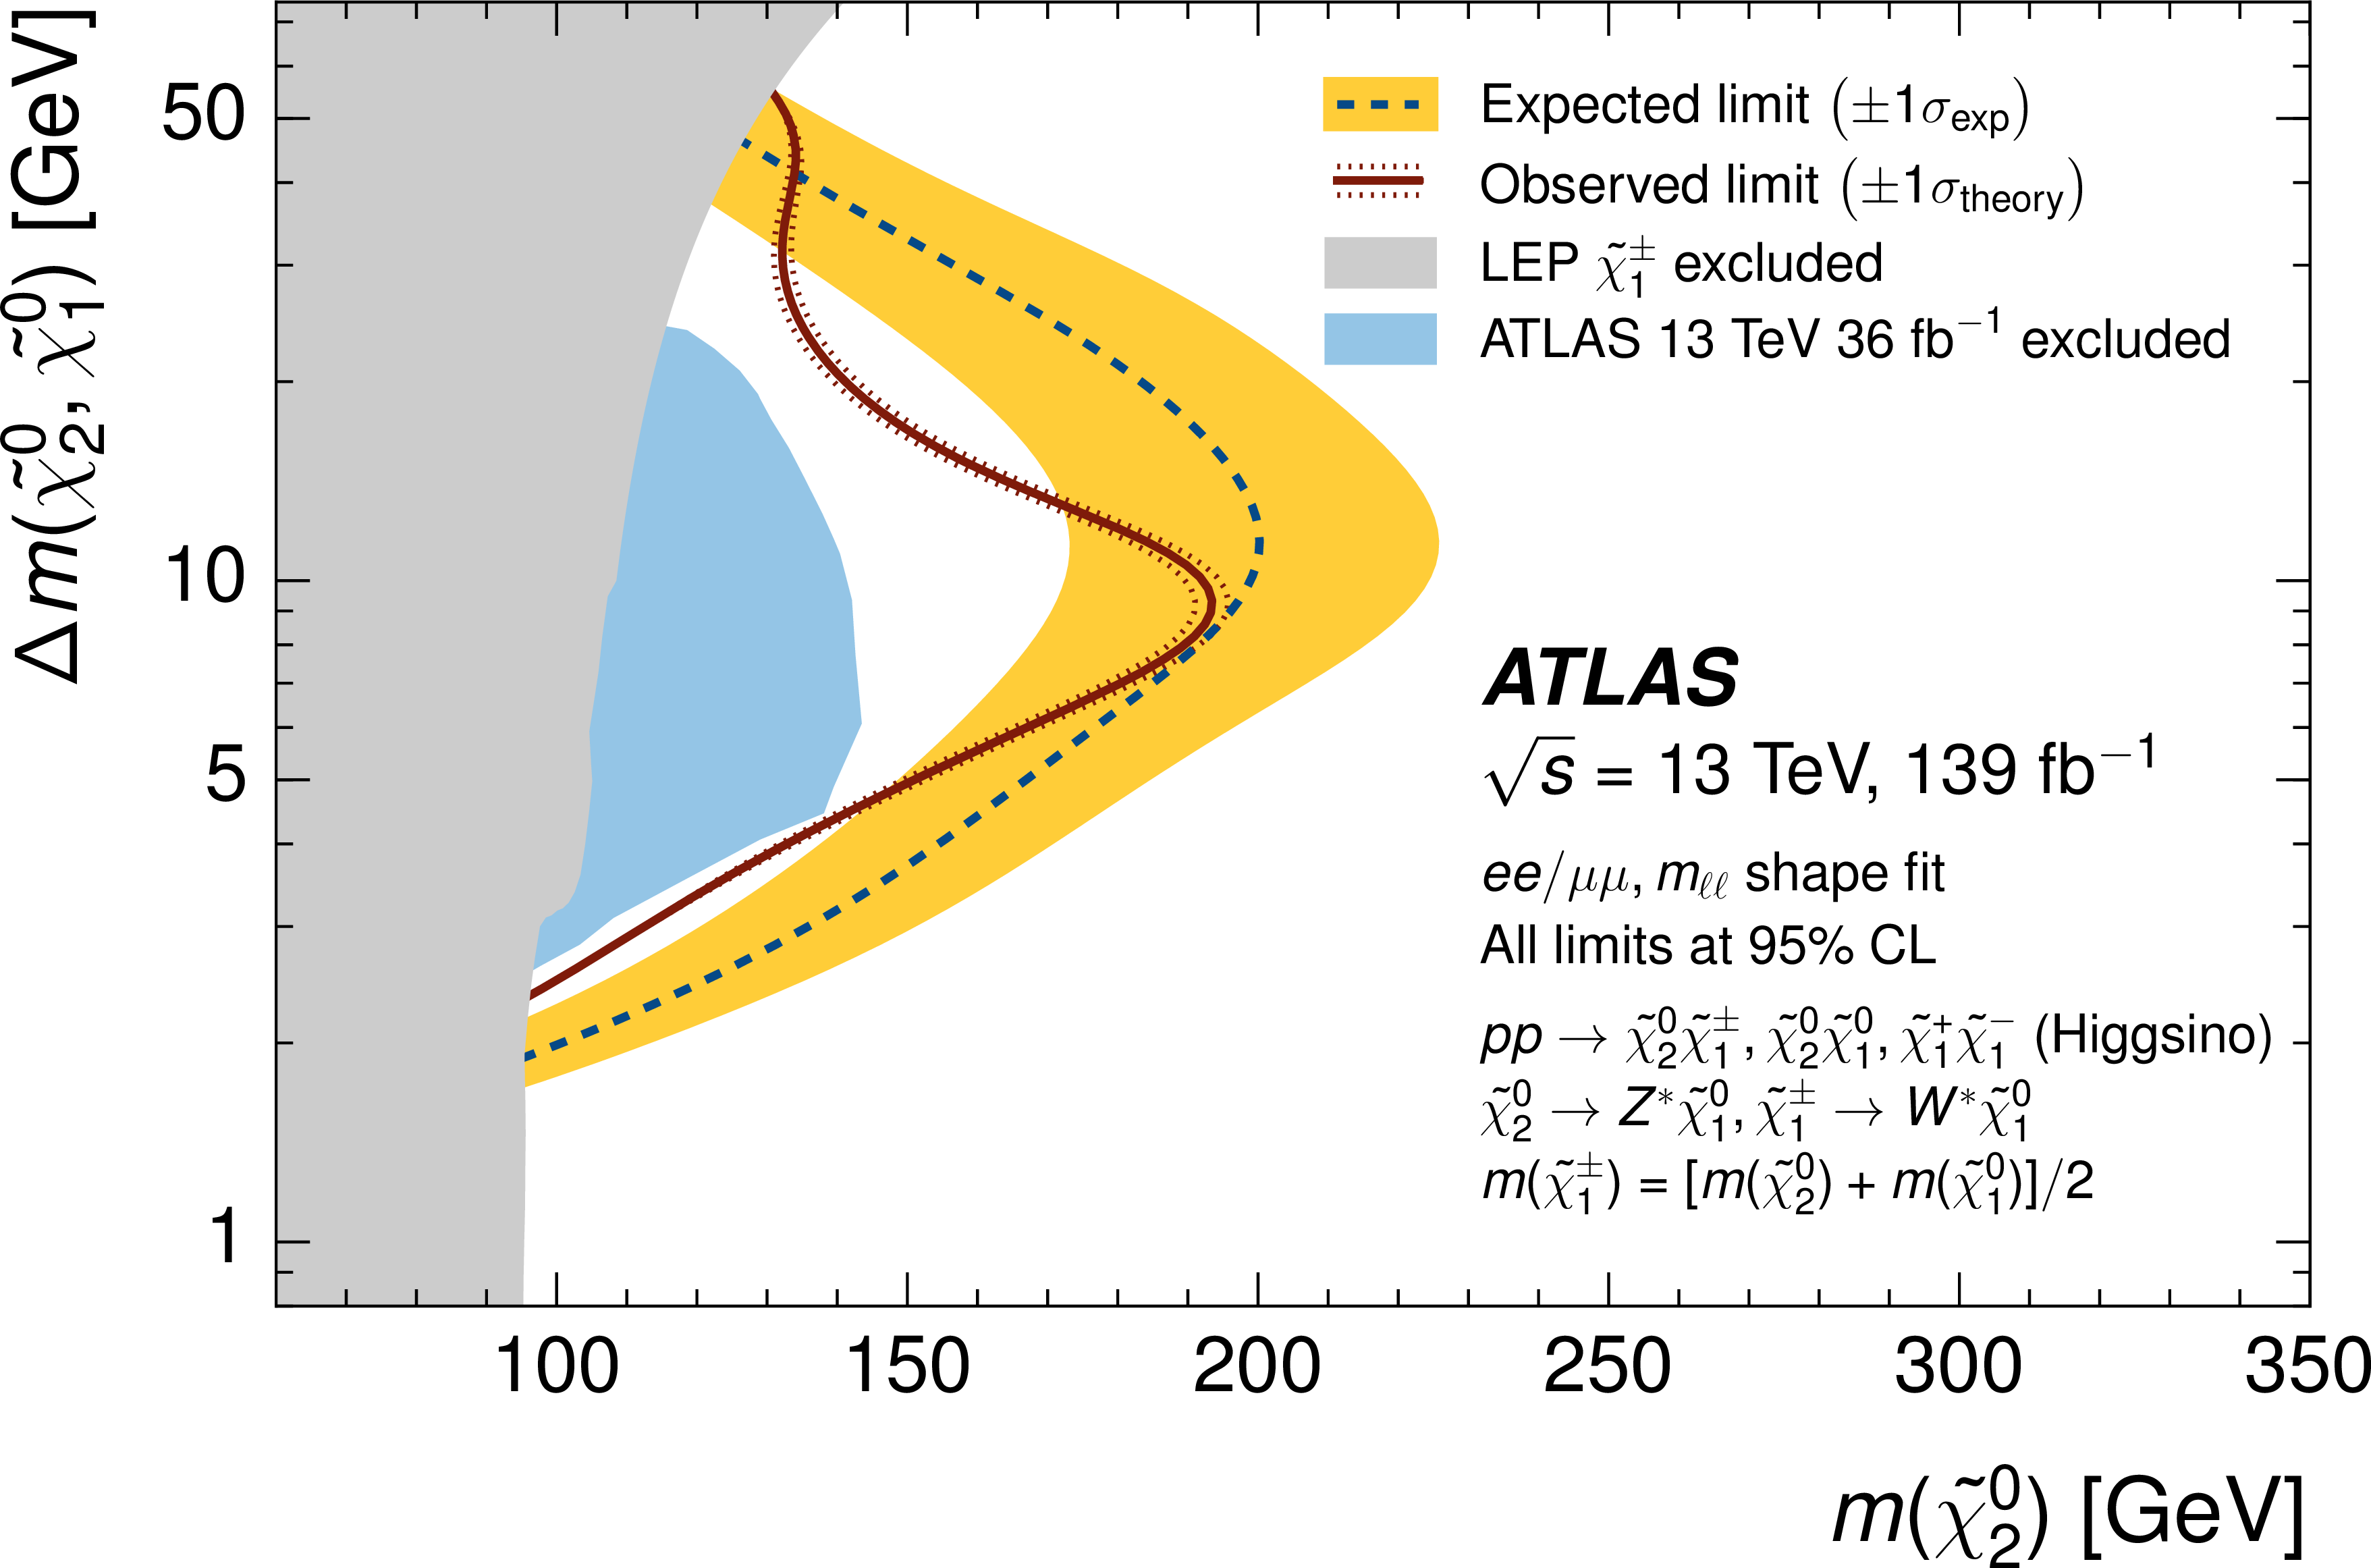
\includegraphics[width=0.48\linewidth]{plots/prev_results/ATLAS_1911_12606.png} \,
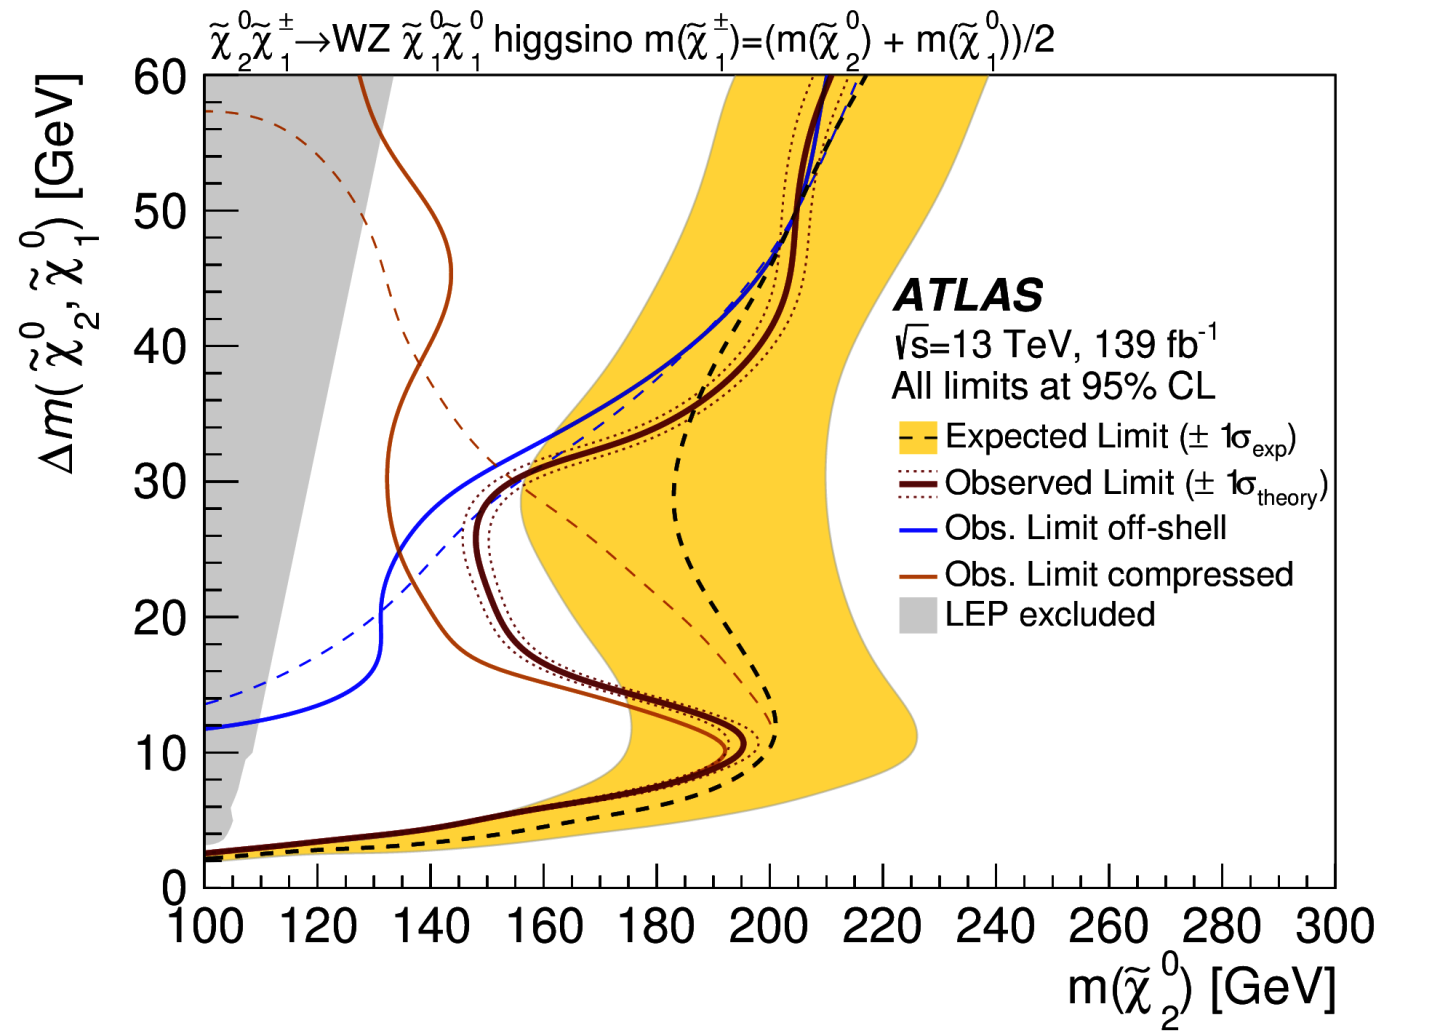
\includegraphics[width=0.48\linewidth]{plots/prev_results/ATLAS-Higgsino-combined_2106_01676.png}  \\
\caption[ATLAS higgsino production exclusion limits]{ATLAS higgsino production exclusion limits for the two lepton final state~\cite{Aad_2020} (left) and combined results for two and three lepton final state~\cite{Aad:2771687} (right).}
\label{fig:atlas-limits}
\end{figure}

At CMS, a search for supersymmetry in final states with two or three soft leptons and missing transverse momentum has been conducted using full Run 2 data~\cite{sos}. This analysis is referred to as SOS, which stands for Soft Opposite-Sign, indicating the final state with two soft opposite-sign same-flavor leptons. Special attention has been given to ensure that the analysis presented in this thesis is orthogonal to the SOS analysis, allowing for a potential future statistical combination. As a result, there is no event overlap between the SOS analysis and the analysis presented in this thesis.

The SOS analysis sets a lower threshold on the transverse momentum of muons, requiring $\pt > 3.5\GeV$. Additionally, it mandates a minimum angular separation between the leptons, with $\DR>0.3$. Section~\ref{sec:signal-signature} provides a detailed exploration of how the analysis presented in this thesis modifies the SOS selection to achieve orthogonality.

In the higgsino simplified model, excluded masses reach up to $205 \GeV$ for a mass splitting $\dm$ of $7.5 \GeV$, and $150 \GeV$ for a highly compressed scenario with $\dm$ of $3 \GeV$. The analysis presented in this thesis aims to extend these exclusion limits towards smaller $\dm$.

\begin{figure}[!htb]
\centering
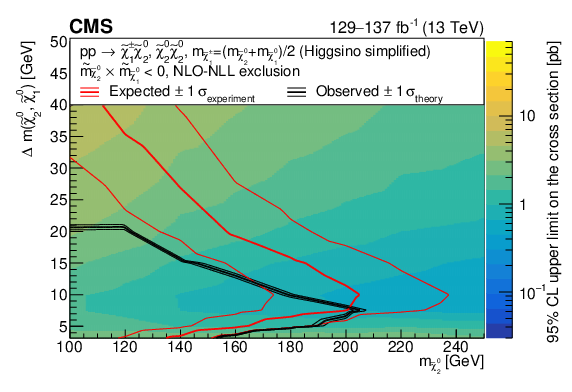
\includegraphics[width=0.80\linewidth]{plots/prev_results/cms_sos_limit.png} \\
\caption[CMS SOS higgsino production exclusion limits]{CMS higgsino production exclusion limits for the SOS analysis of final states with two or three soft leptons in a higgsino simplified model~\cite{sos}.}
\label{fig:cms-sos-limits}
\end{figure}

